\section{Related Work}


\subsection{Linked Data}

Der Begriff \glqq Linked Data\grqq \ beschreibt eine Menge an Prinzipien, wie Daten im Internet strukturiert, publiziert und verlinkt werden sollten. Entwickelt worden sind diese von Tim Berners-Lee, der sie 2006 in seinem Bericht \glqq Linked Data\grqq \ \cite{linked_data} veröffentlichte. Die Grundidee dabei ist, sich dafür die Architektur des Internets zunutze zu machen. Im Wesentlichen handelt es sich dabei um vier Punkte (Übersetzung nach \cite{wiki_linked_data}):
\begin{enumerate}
\item Verwende zur Bezeichnung von Objekten URIs.
\item Verwende HTTP-URIs, so dass sich die Bezeichnungen nachschlagen lassen.
\item Stelle zweckdienliche Informationen bereit, wenn jemand eine URI nachschlägt (mittels der Standards RDF und SPARQL).
\item Zu diesen Informationen gehören insbesondere Links auf andere URIs, über die weitere Objekte entdeckt werden können.
\end{enumerate}

Das erste Prinzip besagt, dass URIs nicht nur benutzt werden sollen, um Dokumente im Internet verfügbar zu machen. Jede Form von Objekten oder Entitäten soll eindeutig über eine URI identifizierbar sein, handele es sich um eine Person, einen spezifischen Gegenstand oder allgemein \glqq Dinge\grqq.


Das zweite Prinzip spezifiert, dass die im ersten Prinzip angesprochenen URIs HTTP-URIs sein sollen. HTTP hat sich im Internet als universales Übertragungsprotokoll etabliert. Die Verwendung von HTTP-URIs ermöglicht es demzufolge, solche URIs einfach nachschlagbar zu machen.


Das dritte Prinzip schlägt die Benutzung eines einheitlichen Formats für die Publikation von Daten vor, in diesem Fall das \glqq Resource Description Framework\grqq \ (RDF)\cite{rdf}. Dabei handelt es sich um ein simples Graph-basiertes Datenmodell. Bei SPARQL\cite{sparql} handelt es sich um eine von SQL inspirierte RDF-Anfragesprache.


Das vierte Prinzip plädiert für die Benutzung von Hyperlinks zur Verlinkung einzelner Ressourcen, um den Zugriff auf weitere thematisch relevante Datenquellen zu ermöglichen. Im Gegensatz zu normalen Hyperlinks, welche keinen Kontext beinhalten, lässt sich bei nach RDF spezifizierten Links ein Kontext angeben. So kann zum Beispiel ausgedrückt werden, dass zwei Ressourcen semantisch äquivalent sind oder dass zwei Personen, die miteinander verlinkt werden, befreundet sind.


\subsection{RDF}

Wie bereits beschrieben, handelt es sich bei RDF um ein Graph-basiertes Datenmodell zur Strukturierung von Daten. Die Daten werden dabei in Tripeln organisiert und bilden einen gerichteten Graphen. Ein Tripel besteht aus Subjekt, Prädikat und Objekt und bildet die Struktur eines simplen Satzes ab. Solch ein simpler Satz könnte wie folgt aussehen:

\begin{lstlisting}
 Led Zeppelin (S) ist (P) eine Band (O).
\end{lstlisting}


Das Subjekt eines Tripels ist eine URI, die die Ressource eindeutig identifiziert. Beim Objekt kann es sich um ein Literal, zum Beispiel eine Nummer oder einen String, oder um eine URI handeln, die mit dem Subjekt in Verbindung steht. Das Prädikat spezifiziert in welcher Form Subjekt und Objekt miteinander in Verbindung stehen. Thematisch zusammenhängende Prädikate werden in so genannten \glqq Ontologien\grqq \ spezifiziert, wobei auch jedes Prädikat über eine URI dereferenzierbar ist.

Der Satz aus dem obigen Beispiel (\glqq Led Zeppelin\grqq \ ist vom \glqq Typ\grqq \ \glqq Band\grqq) wird in der DBpedia folgendermaßen dargestellt\cite{dbpedia_led_zeppelin}:

\begin{lstlisting}
http://dbpedia.org/resource/Led_Zeppelin (S) 
 http://www.w3.org/1999/02/22-rdf-syntax-ns#type (P)
 http://dbpedia.org/ontology/Band (O)
\end{lstlisting}

Hierbei ist noch zu erwähnen, dass URIs, vor allem solche, die öfter vorkommen, im RDF-Format durch Präfixe ersetzt werden können. http://www.w3.org/1999/02/22-rdf-syntax-ns\# wird dann zum Beispiel zum Präfix \glqq rdf:\grqq; Ressourcen aus der DBpedia können durch \glqq dbpedia:\grqq \  dargestellt werden.
Das genannte Beispiel sieht dann derart aus:

\begin{lstlisting}
dbpedia:Led_Zeppelin (S) rdf:type (P) dbpedia-owl:Band (O)
\end{lstlisting}

In dieser Ausarbeitung werden wir der Lesbarkeit halber ebenfalls gängige Präfixe für Ontologien benutzen. Diese sind:
\begin{itemize}
\item dbpprop: \tt <http://dbpedia.org/property/>
\item dbpedia-owl: \tt <http://dbpedia.org/ontology/>
\item rdf: \tt <http://www.w3.org/1999/02/22-rdf-syntax-ns\#>
\item rdfs:\tt <http://www.w3.org/2000/01/rdf-schema\#>
\item mo: \tt <http://purl.org/ontology/mo/>
\item foaf: \tt <http://xmlns.com/foaf/0.1/>
\item owl: \tt <http://www.w3.org/2002/07/owl\#>
\end{itemize}



\subsection{DBpedia}

Bei der DBpedia handelt es sich um ein offenes Projekt, dessen Ziel es ist, die in der Wikipedia zusammengetragenen Daten nach der RDF Spezifikation zu strukturieren und unter offener Lizenz zu veröffentlichen \cite{dbpedia_about}. Sie besteht seit 2007 und ist eines der größten Projekte, das sich mit Linked Data befasst. Aufgrund ihrer Größe, des breiten Spektrums an Informationen, welche abgedeckt werden, und der Anzahl der Verlinkungen zu anderen Datensätzen, bildet die DBpedia einen großen Knotenpunkt im Web of Data und ist demzufolge eine gute Grundlage für die Erstellung eines Linked Data Mashups (siehe Abb. 1).

\begin{figure}[ht!]
	\centering
	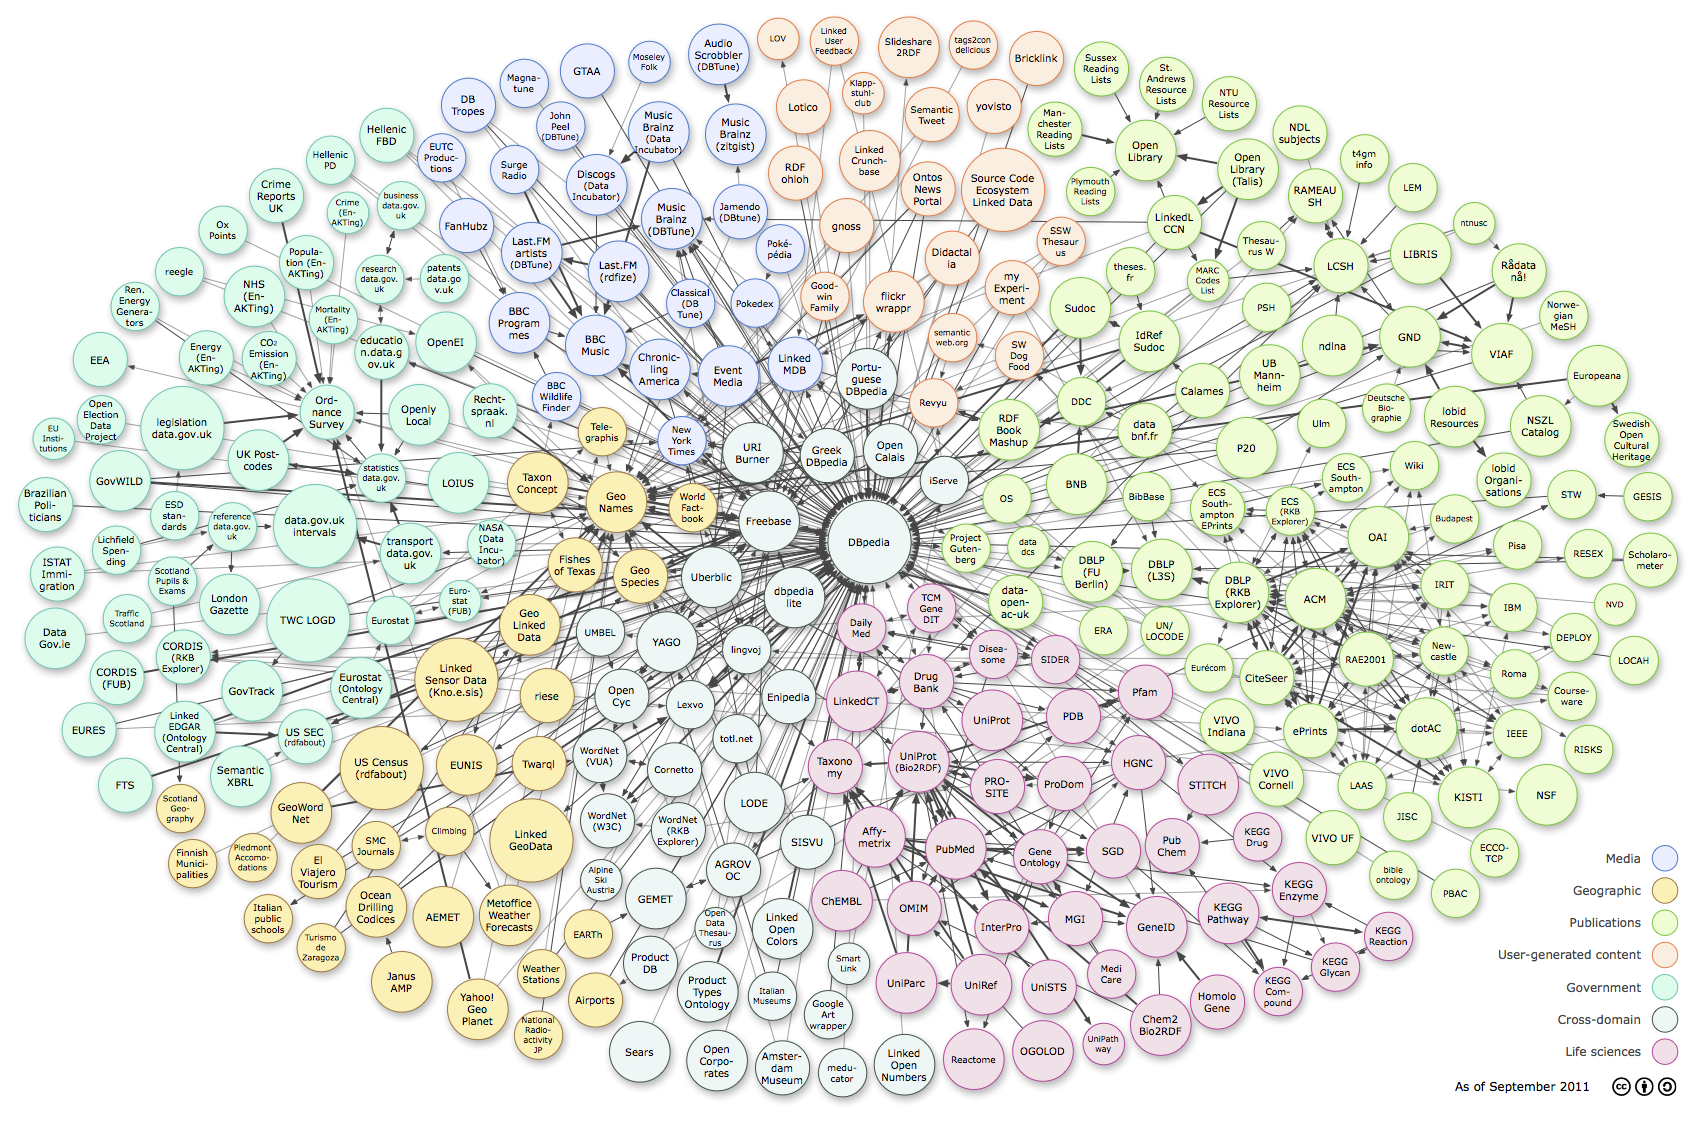
\includegraphics[width=120mm]{bilder/ldcloud.jpg}
	\caption{Die \glqq Linked Data Cloud\grqq \ \cite{linked_data_cloud} \label{overflow}}
\end{figure}

\subsection{Existierende Empfehlungsdienste}
\paragraph{} Seitdem Musik gemacht und verkauft wird, besteht auch immer ein Bedarf danach neue Musik zu entdecken, die einem gefällt. Was früher nur durch das Gespräch mit Freunden oder im Plattenladen möglich war, wird heute auch automatisiert im Internet angeboten.

\paragraph{} Man unterscheidet dabei zwischen \textbf{inhaltsbasierten} und kollaborativen Empfehlungsdiensten. Bei ersteren steht die Musik selbst im Mittelpunkt; ausgehend von einem Musikstück oder einer Band wird bestimmt, welche anderen Bands und Lieder diesem ähnlich sind, zum Beispiel durch ein ähnliches Genre oder gemeinsame Mitglieder.

\paragraph{} \textbf{Kollaborative} Empfehlungsdienste dagegen betrachten nicht die Musik als solche, sondern arbeiten mit Statistiken auf Basis der Interaktionen ihrer Nutzer. Ein einfaches Beispiel stellt gnoosic\footnote{\url{http://www.gnoosic.com/}} dar, das nach der Eingabe eines Interpreten weitere vorschlägt, für die man jeweils angeben kann, ob man diese ebenfalls mag. 

Der Nutzen dieser Dienste entsteht durch die große Menge an nutzergenerierten Informationen. Durch die Auswertung des Geschmacks vieler Leute lässt sich meist eine präzise Aussage treffen, ob der Hörer von Band A auch Band B schätzt.

\paragraph{} Daneben gibt es auch \textbf{nicht-automatische Varianten} der Musikempfehlung, zum Beispiel durch Freunde, in Musikgeschäften oder Zeitschriften.

\paragraph{} Viele Empfehlungsdienste sind direkt in andere Dienste integriert, so zum Beispiel beim Online-Händler Amazon\footnote{\url{http://www.amazon.com/}} oder dem Musikstreamingportal Spotify\footnote{\url{http://www.spotify.com/}}. Diese werten direkt das Kauf- bzw. Hörverhalten ihrer Kunden aus, um damit Empfehlungen zu generieren.  

Außerdem existieren spezialisierte Empfehlungsdienste, so zum Beispiel der BibTip-Service des Karlsruher Instituts für Technologie\footnote{\url{http://www.bibtip.com/}} oder Webseiten wie TasteKid\footnote{\url{http://www.tastekid.com/}} und Musicovery\footnote{\url{http://musicovery.com/}}. Wiederum andere Dienste richten sich an spezielle Anwendungszwecke wie Jog.fm\footnote{\url{https://jog.fm/}}, dass je nach Laufgeschwindigkeit die musikalische Untermalung zum Joggen empfiehlt.

Neben den genannten Beispielen lassen sich für jede Kategorie weitere Anbieter finden, auf die jedoch nicht näher eingegangen werden soll.

\paragraph{} Im \textbf{Vergleich} zum vorgestellten Ansatz existieren zwei signifikante Unterschiede. Zum ersten gibt keines der anderen Musikempfehlungssysteme Gründe an, warum bestimmte Interpreten empfohlen werden. Zum zweiten verfolgen die anderen Systeme jeweils einen Ansatz gezielt, haben also zum Beispiel Musik, aber keine Liste anstehender Konzerte oder einen Abstract über den Interpreten. MusicMashup gibt Gründe für die Empfehlungen an und bietet neben der Empfehlungslogik auch weitere Funktionalität an. Wie dies im Detail geschieht, wird im nächsten Kapitel genauer beschrieben.